%%%%%%%%%%%%%%%%%%%%%%%%%%%%%%%%%%%%%%%%%%%%%%%%%%%%%%%%%%%%%%%%%%
%%This presentation was fullly copied from the WSC presentation (dec. 2015)
%% and addapted for the CAA2k16
%% and then  for the EPNET workshop of the 3rd of may
\documentclass[12pt, notes=show]{beamer}
\usetheme[width=0cm]{Goettingen}
\usecolortheme{rose}
\useoutertheme{default}
\setbeamerfont{caption}{size=\scriptsize}
\setbeamertemplate{navigation symbols}{}

\addtobeamertemplate{navigation symbols}{}{%
	\usebeamerfont{footline}%
	\usebeamercolor[fg]{footline}%
	\hspace{1em}%
	$\dfrac{\insertframenumber}{\inserttotalframenumber}$
}

\usepackage{fontspec} 
\setsansfont{Futura LT}
%\setmonofont[Scale=0.8]{Monaco} 


\usepackage{arydshln}

\usepackage{amsmath}

\usepackage{mathptmx}
\usepackage{latexsym}
\usepackage{mathtools}
\usepackage{caption}
\usepackage{array}




\title{
	Co-evolution of trade and culture\\
	Impact of cultural network topology on economic dynamics.
}

\institute{10 May 2016}

\author{Simon Carrignon, Jean-Marc Montanier, Jérôme Michaud, Xavier Rubio-Campillo \& Ignacio Morer }

\date{
	\scriptsize
	\begin{columns}
		\begin{column}{.3\textwidth}
			\begin{center}
				Barcelona Supercomputing Center	\\
				
\includegraphics[height=1cm]{images/bscLogo.jpg} \hspace{2cm}
			\end{center}
		\end{column}
		\begin{column}{.3\textwidth}
			\begin{center}
				Univ. Pompeu Fabra Complex System Lab.\\
				\includegraphics[height=1cm]{images/upfLogo.jpeg} %declare logo image with an alias here 
			\end{center}
		\end{column}
	\end{columns}

}
\begin{document}
\begin{frame}
	\maketitle

\end{frame}

\section{Introduction}

\begin{frame}{Cultural Evolution}
    Social Traits:
    \begin{center}
	\begin{table}
	    \center
	    \begin{tabular}{ccc}
		\uncover<2->{\includegraphics[height=3cm]{images/m80}} &
		\uncover<3->{\includegraphics[height=3cm]{images/m90}} &
		\uncover<4->{\includegraphics[height=3cm]{images/m10}} \\
		\uncover<2->{80's} & \uncover<3->{90's} & \uncover<4->{now}
	    \end{tabular}
	\end{table}
    \end{center}
    \uncover<5->{How they Evolve?}\uncover<6>{ Cultural Evolution }
\end{frame}


\begin{frame}{Cultural Evolution}
    \begin{itemize}
	\item<5->{ culturally transmitted, socially learnt}
	\item<6->{ similar patterns}
    \end{itemize}
	\begin{center}
		\uncover<4->{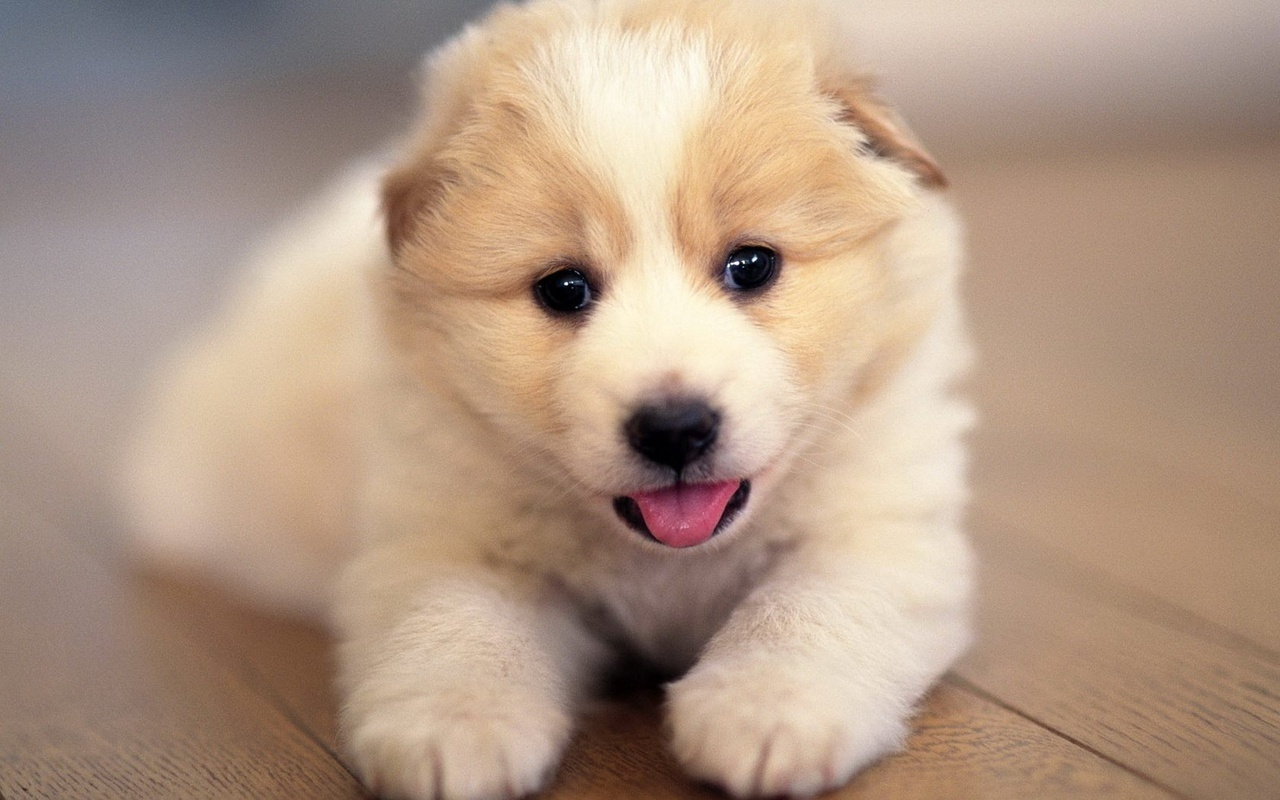
\includegraphics[width=3cm]{images/cutdog}}\\
		\vspace{.5cm}
		\uncover<2->{\includegraphics[width=2.5cm]{images/cutbaby}}
	    \hspace{1cm}
	    \uncover<3->{ \includegraphics[width=2cm]{images/pottery}}
	\end{center}
    \uncover<7>{$\rightarrow$ What mechanism drive the evolution of such traits?\\
    \invisible<1->{$\rightarrow$ What mechanism }generate such pattern?}
\end{frame}

\begin{frame}{What Generate Those Cultural changes?}
	Simple mechanisms (Bentley et al, 2004):
	\begin{itemize}
		\item<2->Random Copy 
		\item<3-> Frequency biased (conformist/anti-conformist\dots)
		\item<4->\dots	
	\end{itemize}
	\uncover<2>{\begin{figure}
		\begin{columns}
			\begin{column}{.8\textwidth}
				\centering
				\includegraphics[width=.6\textwidth]{images/powerlawrepartition.jpg}
			\end{column}
			\begin{column}{.3\textwidth}
				\tiny
				Square: male names\\
				Circle: female names\\
				Dotted and plain lines: model result with different copy probabilities.\\
			From Bentley et al,~2004.
			\end{column}
		\end{columns}
	    \end{figure}}
\end{frame}

\section{Context}

\begin{frame}
	\only<1->{\begin{center}
	    What if such mechanisms act on traits linked to economics?
    \end{center}}
	\begin{center}
	    \only<2>{\includegraphics[height=4cm]{images/tools}}
	    \only<3>{\vspace{1cm}\includegraphics[height=3cm]{images/bordeaux.jpg}\hspace{2cm}
	    \includegraphics[height=3cm]{images/napa}}
	    \only<4-7>{
		    \uncover<4->{\includegraphics<4-5>[height=4cm]{images/social1.png}\includegraphics<6->[height=4cm]{images/social2.png}}
		    \uncover<5->{{  \Large \only<5>{$\rightarrow$} \only<6>{$\leftarrow$}\only<7>{$\leftrightarrow$}}}
	    \uncover<5-7>{\includegraphics<5-6>[width=.4\textwidth]{images/eco.png} \includegraphics<7>[width=.4\textwidth]{images/eco2.png}}

    		}
	\end{center}
\end{frame}
\begin{frame}
	\begin{center}
		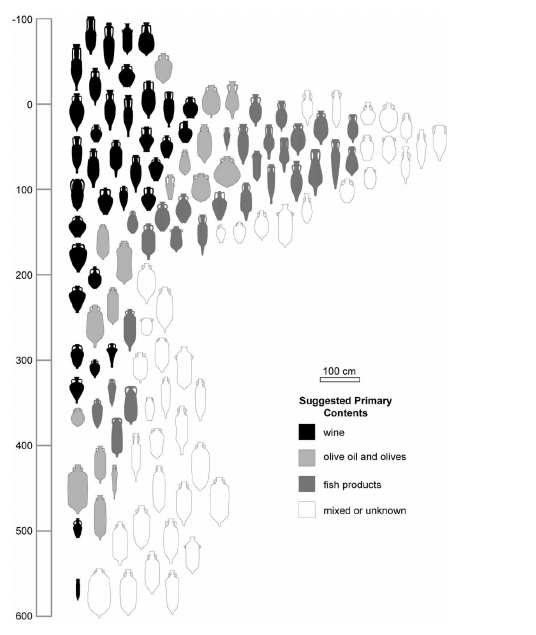
\includegraphics[height=\textwidth]{images/bevan.png}
	\end{center}
\end{frame}

\begin{frame}{Co-evolution of Economy and Culture}

%How Simple Cultural Dynamics influence Economy That in turn will influence cultural dynamics.
    \begin{center}
	\includegraphics[width=\textwidth]{images/interaction}	
    \end{center}

\end{frame}


\section{ABM Framework}


\begin{frame}{A General Agent Based Framework }

	Two main components:
	\vfill
	\begin{enumerate}
		\item Trade side: Bartering Economy (Gintis 2009),
			\vspace{1cm}
		\item Cultural side: ``copy the most successful'' (Bentley 2006).
	\end{enumerate}

\end{frame}

\begin{frame}{The Model}
	\begin{block}{1. The Economy \& the Barter Mechanism}
		\begin{itemize}
			\item $N$ goods
			\item $M$ Agent 
				$\left\{
					\begin{tabular}{@{}l@{}}
						a quantity of each Goods \\
						$N$ values attributed to each goods\\
					\end{tabular}
					\right.$
				\item Agents \emph{produce} one good and \emph{exchange} it to obtain the other goods.
				\item After the exchange, the agents \emph{consume} all goods 
			\end{itemize}
			Agent perform this 10 times and a scores is given to each of them.
		\end{block}
	\end{frame}

	\begin{frame}{The Model}
		\begin{block}{2. Cultural Mechanisms}
			\begin{itemize}
					\vfill
				\item Less successful agents \emph{copy} the most successful (Biased-Copy).
					\vfill
				\item Given a probability $\mu$ the value attributed to some goods is modified (Innovation/Mutation)
			\end{itemize}
		\end{block}
	\end{frame}

	\begin{frame}{The Model }

		\begin{figure}
			\caption{Example for 3 goods and 600 agents}
			\begin{columns}
				\column{.5\textwidth}
				\includegraphics[width=5cm]{images/full.pdf} 
							%\caption{Evolution of the score of the agents in a setup with 600 agents and 3 goods trading and exchanging their strategies during 10000 timesteps.}%%
			\end{columns}
			@~Equilibrium: mean of score  $\rightarrow$ score max (Carrignon et al. 2015)
		\end{figure}

	\end{frame}

	\section{Experimental Setup \& Results}
	\begin{frame}{Experiments}
		\textbf{Impact of the topology of the cultural network }
		\begin{center}
			``What properties of the cultural network influence the economic dynamics? '' 
		\end{center}
		\begin{center}
			\includegraphics<1>[trim={2cm 6cm 2cm 5cm},clip,width=6cm]{images//trade-cultural.png}
			\includegraphics<2->[trim={2cm 6cm 2cm 5cm},clip,width=6cm]{images//trade-cultural2.png}
		\end{center}
		\vfil
		\uncover<3>{$\rightarrow$ Average Distance vs Average Degree}




	\end{frame}


	\begin{frame}{Degree}
		\begin{center}
			\includegraphics<1>[height=.9\textheight]{images/hmA.png} 	
			\includegraphics<2>[height=.9\textheight]{images/hmAneighbours} 	
			\includegraphics<3>[height=.9\textheight]{images/hmAk4.png} 	
			\includegraphics<4>[height=.9\textheight]{images/hmB.png} 	
			\includegraphics<5>[height=.9\textheight]{images/hmBneighbours} 	
			\includegraphics<6>[height=.9\textheight]{images/hmBk4.png} 	
		\end{center}
	\end{frame}
	\begin{frame}{Shortest Path Length}
		\begin{center}
			\includegraphics<1>[height=.9\textheight]{images/hmA.png} 	
			\includegraphics<2>[height=.9\textheight]{images/hmAB.png} 	
			\includegraphics<3>[height=.9\textheight]{images/hmABlinked.png} 	
			\includegraphics<4>[height=.9\textheight]{images/hmABlinkedL25.png} 	
			\includegraphics<5>[height=.9\textheight]{images/hmCDL6.png} 	
		\end{center}
	\end{frame}
	\begin{frame}{Degree}
		\begin{center}
			\includegraphics<1>[height=.9\textheight]{images/smA.png} 	
			\includegraphics<2>[height=.9\textheight]{images/smAneighbours} 	
			\includegraphics<3>[height=.9\textheight]{images/smAk9.png} 	
		\end{center}
	\end{frame}
	\begin{frame}{Shortest Path Length}
		\begin{center}
			\includegraphics<1>[height=.9\textheight]{images/smA.png} 	
			\includegraphics<2>[height=.9\textheight]{images/smAB.png} 	
			\includegraphics<3>[height=.9\textheight]{images/smABlinked.png} 	
			\includegraphics<4>[height=.9\textheight]{images/smABlinkedL4.png} 	
		\end{center}
	\end{frame}
%	\\Trade Mechanism + Success Biased Copy\\
%	\vfill
%	vs\\
%	\vfill
%	\textbf{Neutral Model}\\ Trade Mechanism + Random Copy\\

	\begin{frame}{Experimental Setup}
		Set of networks with combination of properties:
		\begin{itemize}
			\item Average Degree (D)
			\item Average Distance (A)
		\end{itemize}
		\begin{center}
			\begin{tabular}{l|ccc}
				& $\left\langle k \right\rangle_1$ & \dots & $\left\langle k \right\rangle_n$\\
				\hline\\
				$L_1$	& $G_{11}$	& 	& $G_{1n}$	\\	
				\dots	&		&\dots	&		\\
				$L_m$	& $G_{m1}$	& 	& $G_{mn}$	\\	
			\end{tabular}
		\end{center}

	\end{frame}
	\begin{frame}{Experimental Setup}
		\begin{table}
			\centering
			\begin{tabular}{m{1.2cm}m{2.5cm}m{2.5cm}}
				&$\left\langle k\right\rangle=8$ & $\left\langle k\right\rangle=4$\\
				$L\approx17$&
				\includegraphics[width=2.5cm]{images/g02.pdf}&
				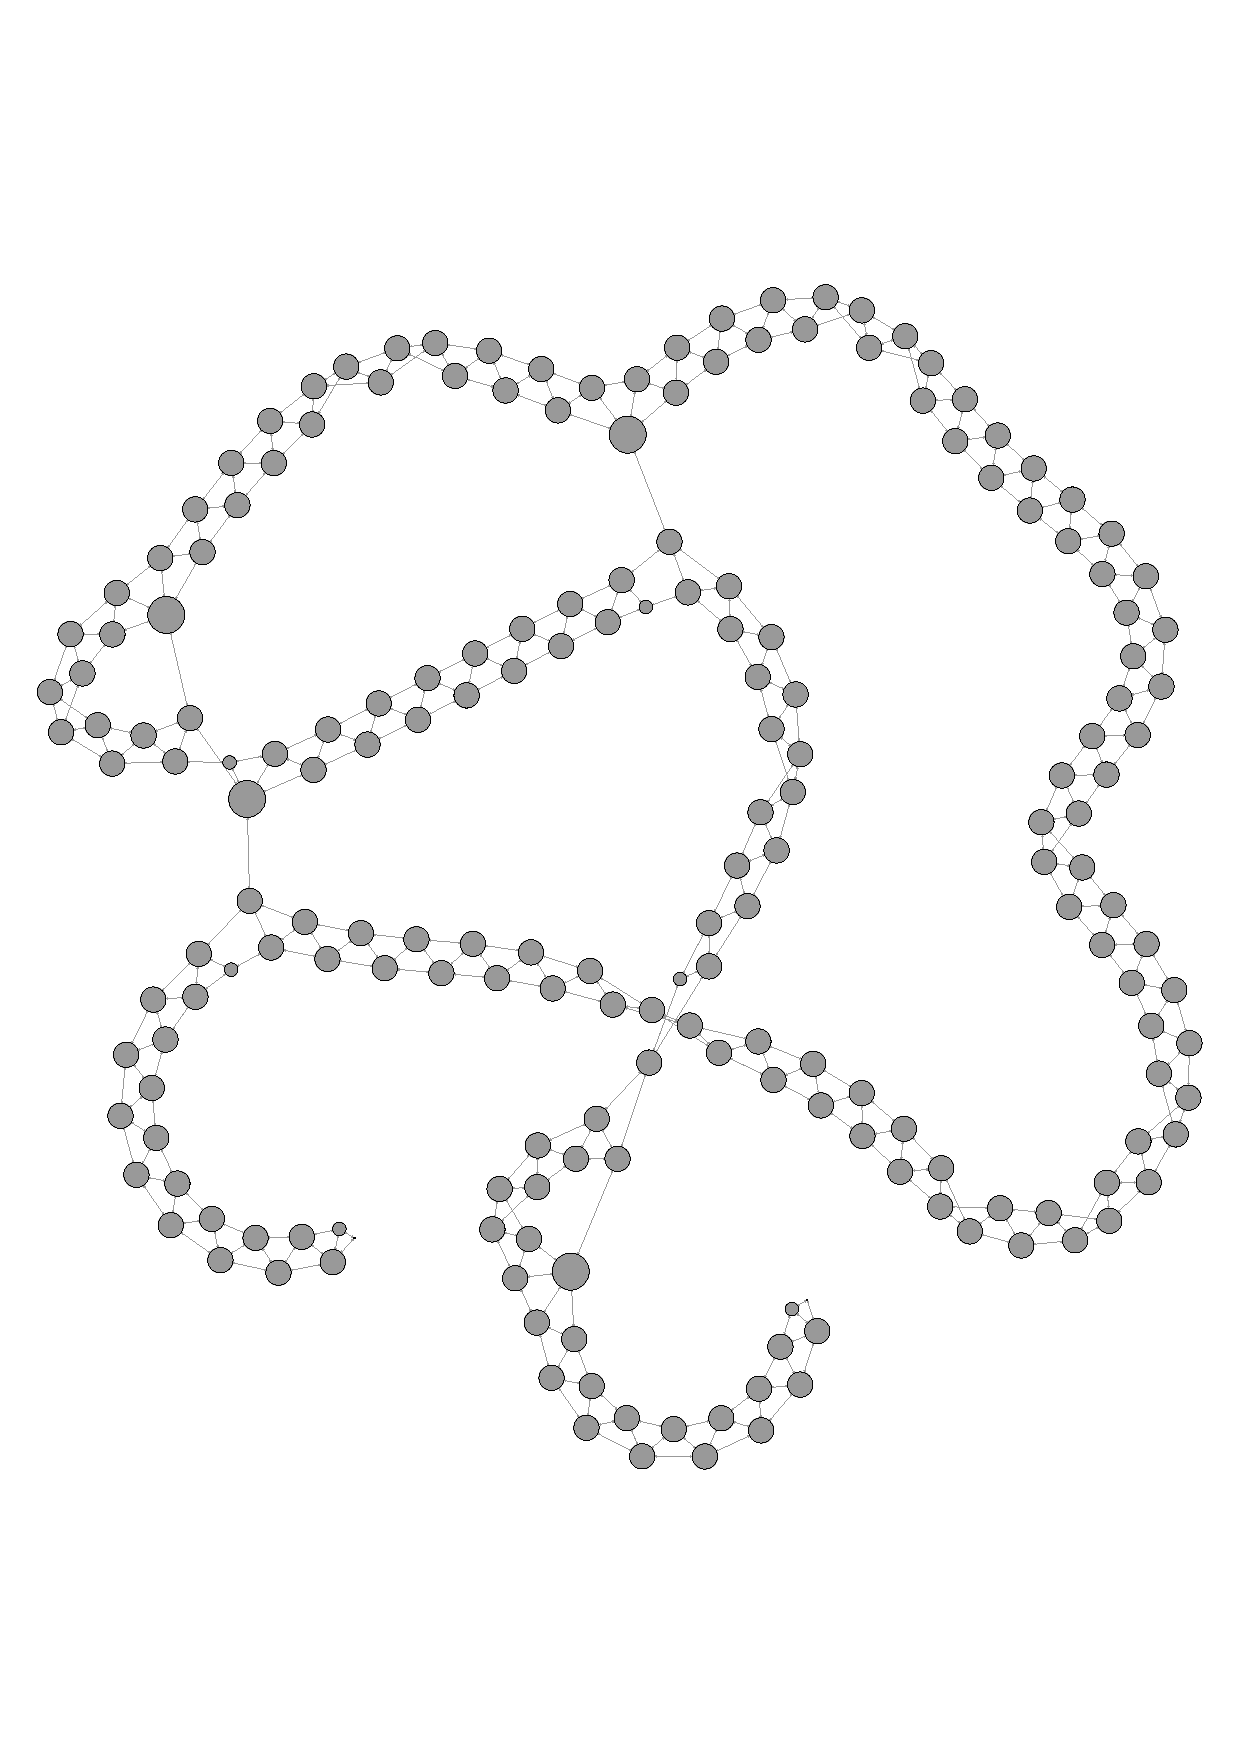
\includegraphics[width=2.5cm]{images/g00.pdf}\\
				$L\approx4$&
				\includegraphics[width=2.5cm]{images/g42.pdf}&
				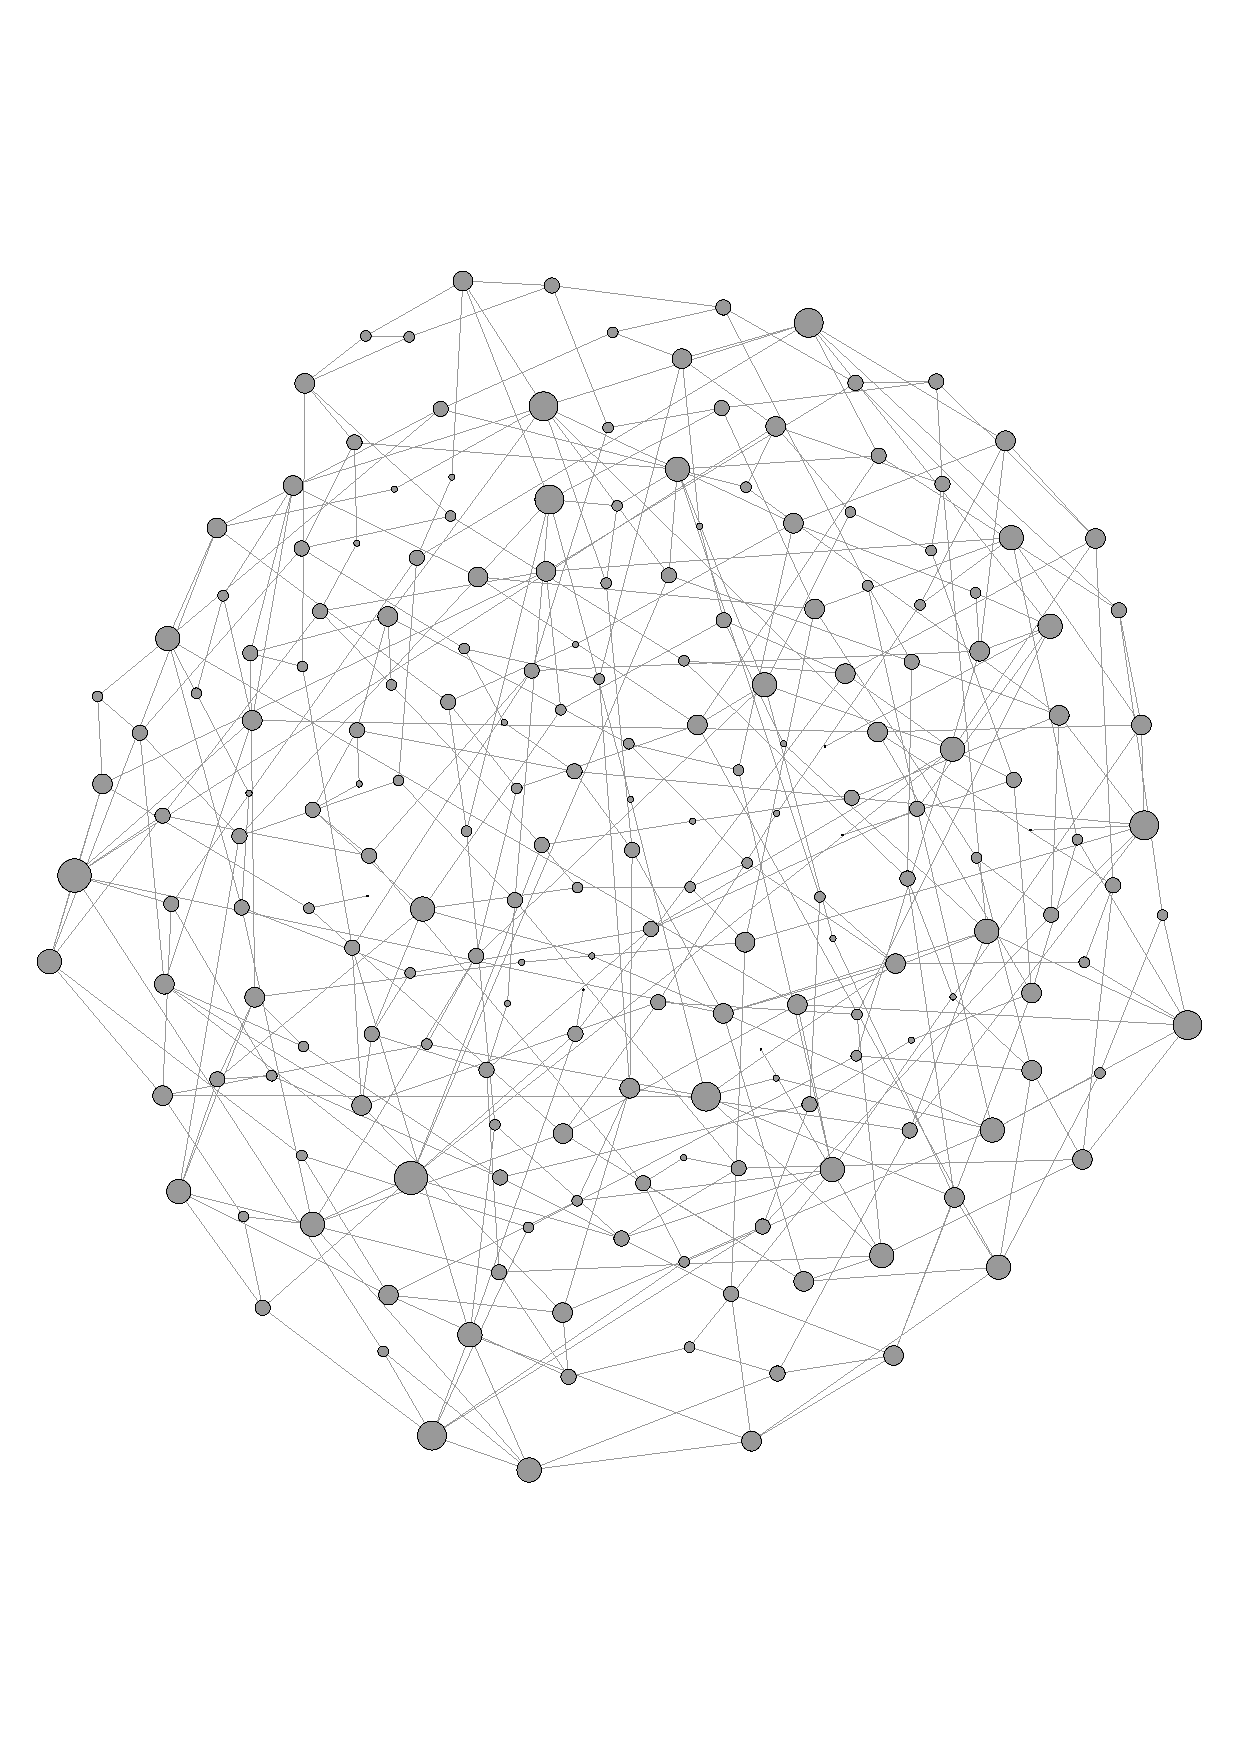
\includegraphics[width=2.5cm]{images/g40.pdf}\\
			\end{tabular}
		\end{table}
	\end{frame}



	\begin{frame}{Results: }
		General Behaviour of the simulations with different topologies.
		\begin{figure}[h]
			\begin{center}
				\includegraphics[height=.5\textheight]{images//provResults2.pdf}
			\end{center}
		\end{figure}

	\end{frame}

	\begin{frame}{Results: }
		\begin{figure}[h]

			Time of convergence as a function of $L$.
			\begin{center}
						%Behaviour of the simulations with different topologies.}
				\includegraphics[height=.6\textheight]{images//L_vs_t10.pdf}

			\end{center}
		\end{figure}

	\end{frame}

	\begin{frame}{Results: }
		\begin{itemize}
				\vfill
			\item Average Degree doesn't seem to have much impact
				\vfill
			\item Average Distance speed up the convergence
		\end{itemize}

	\end{frame}



	\begin{frame}{Conclusion}
		\begin{itemize}
			\item Simple cultural mechanism and simple trade can lead to efficient economic dynamics:\\
				{$\rightarrow$ \small Both aspect should be studied together.}
				\vfill
			\item Properties of the cultural network impact thoses dynamics.\\
				{$\rightarrow$\small Different network support different economy}
				\vfill
		\end{itemize}

	\end{frame}
	\begin{frame}{}
		\begin{center}
			\huge
			Thank for you attention!\\
		\end{center}


	\end{frame}

	\end{document}


